\documentclass[12pt,a4paper]{report}
\usepackage[T1]{fontenc}
\usepackage{newtxmath,newtxtext}
\usepackage{indentfirst}     % Отступ в первом абзаце
\renewcommand{\baselinestretch}{1.0} 


\pagestyle{empty}
\usepackage[left=2.5cm, right=1.5cm, top=2.5cm, bottom=2.5cm]{geometry}
\usepackage[medium]{titlesec}
\usepackage{graphicx}
\usepackage{float}
\usepackage{array,caption}
\usepackage{listings}
\usepackage{hyperref}
\graphicspath{ {./images/} }

\lstset{language=python, frame = single}  
\lstset{numbers=left, numberstyle=\tiny, numbersep=5pt, breaklines=true, basicstyle=\small}  
%\lstset{emph={square}, emphstyle=\color{red}, emph={[2]root,base}, emphstyle {[2]\color{blue}}}

\begin{document}
	\vspace*{15ex}
	\begin{center}
		FEDERAL STATE AUTONOMOUS EDUCATIONAL INSTITUTION OF HIGHER EDUCATION 
		
		ITMO UNIVERSITY
		\vspace*{30ex}
		
		Report\\
		on the practical task No. 2\\
		``Algorithms for unconstrained nonlinear optimization. Direct methods``
	\end{center}
	\vspace{25ex}
	\begin{flushright}
		Performed by\\
		Maxim Ryazanov\\
		J4133c\\
		Accepted by\\
		Dr Petr Chunaev
	\end{flushright}
	\vspace{20ex}
	\begin{center}
		St. Petersburg\\
		2021
	\end{center}
	\newpage

    \section*{Formulation of problem}

\subsection*{Goal}
The use of first- and second-order methods (Gradient Descent, Non-linear Conjugate Gradient Descent, Newton's method and Levenberg-Marquardt algorithm) in the tasks of unconstrained nonlinear
optimization
\subsection*{Subtasks}
\textbf{I.} Generate random numbers $\alpha \in (0, 1)$ and $\beta \in (0, 1)$. Furthermore, generate the noisy data ${x_k, y_k}$, where $k = 0, ..., 100$ according to the following rule:

\begin{equation*}
    y_k = \alpha x_k + \beta + \delta_k, x_k = \frac{k}{100}
\end{equation*}

where $\delta_k \sim N(0, 1)$ are values of random variable with standard normal distribution. Approximate the data by the following linear and rational functions:

\begin{enumerate}
    \item $F(x, a, b) = ax + b$,
    \item $F(x, a, b) = \frac{a}{1 + bx}$,
\end{enumerate}

by means of least squares through the numerical minimization (with precision $\epsilon = 0.001$) of the following function:

\begin{equation*}
    D(a, b) = \Sigma_{k=0}^{100} (F(x_k, a, b) - y_k)^2.
\end{equation*}

To solve the minimization problem, use the methods of Gradient Descent, Non-linear Conjugate Gradient Descent, Newton's method and Levenberg-Marquardt algorithm. If necessary, set the initial approximations and other parameters of the methods.
Visualize the data and the approximants obtained in a plot seperately for each type of approximant.
	\section*{Theory}

Optimization methods are the methods for finding optimal (in some sense) sollutions
for mathematical models which are usually expressed via an objective function $f = f(x)$, where $x$ is generally a multidimensional vector.

To solve the optimization problem $f(x) \rightarrow min_{x\in Q}$ means to find $x^{*} \in Q$ where $Q$ is the region of acceptability, such  that $f$ reaches the minimal value at $x^{*}$.

For unconstrained optimization methods (which are used in this work) the region of acceptability $Q$ is not defined.

\subsection*{Direct methods}
\subsubsection*{Nelder-Mead}

This method uses simplexes in $R^n$. In our case ($n = 2$), they are triangles.

This is an heuristic approach wich can stuck in a local minima or cnverge to non-stationary point.
The method consists of 7 main steps:
\begin{enumerate}
    \item \textbf{Preparation.} Three points for triangle are choosed ($x_1, x_2, x_3$) and function value is calculated for these points.
    \item \textbf{Sorting.} Points are choosen that $x_h$ with largest $f_h$, $f_g$ with $x_g$ and the lowest $f_l$ and $x_l$.
    \item \textbf{Gravity centre.} The gravity centre for the lowest points is calculated $x_c = \frac{1}{2}(x_g + x_l)$
    \item \textbf{Reflection.} The point $x_h$ is reflected with respect to $x_c$.
    \item \textbf{Expansion.} Check weather the dirrection of reflection is right and simplex can be moved in that dirrection. Otherwise, go to step 6.
    \item \textbf{Shrinking.} Shrinks the simplex globally.
    \item \textbf{Convergence check.} Check the mutal closeness of simplex vertices. If the required precision is not achieved, go to Step 2.
\end{enumerate}

\subsection*{Second-order methods}
\subsubsection*{Levenberg-Marquardt algorithm (LMA)}

The LMA is a pseudo-second order method, its application is to solve non-linear least squares problems.

For a set $(x_i, y_i)^{m}_{i=1}$, find a column-vector $\beta^{*}$ of the parameters $\beta = (\beta_1, ..., \beta_n)^T$ of the function $f(x, \beta)$ such that

\begin{equation*}
    \beta^{*} = arg min_{\beta} S(\beta), S(\beta) = \Sigma_{i=1}^m (y_i - f(x_i, \beta))^2
\end{equation*}

Start with an initial guess for $\beta$. At each iteration, $\beta$ is replaced  $\beta + \Delta \beta$. To determine $\Delta \beta$, $f(x_i, \beta)$ is approximated by its linearization:
\begin{equation*}
    f(x_i, \beta + \Delta \beta) \approx f(x_i, \beta) + J_i \Delta \beta
\end{equation*}

\begin{equation*}
    J_i = (\frac{\partial f(x_i, \beta_j)}{\partial \beta_j})_{j=1}^n
\end{equation*}

$J_i$ is a row-vector.

The sum $S(\beta)$ has its minimum at a zero gradient with respect to $\beta$. The above-mentioned linear approximation of $f(x_i, \beta + \Delta \beta)$ gives

\begin{equation*}
    S(\beta + \Delta \beta) \approx \Sigma_{i=1}^m (y_i - f(x_i, \beta) - J_i \Delta \beta)^2
\end{equation*}

or in a vector notation,

\begin{equation*}
    S(\beta + \Delta \beta) \approx (y - f(\beta))^T(y - f(\beta)) - 2(y - f(\beta))^TJ\Delta \beta + \Delta \beta^TJ^TJ\Delta\beta
\end{equation*}

where $J$ is the Jacobian matrix, whose $i$-th row equals $J_i$, and where $f(\beta)$, $y$ and $\beta$ are column-vectors with $i$-th component $f(x_i, \beta), y_i, \beta_i$ respectively.

Taking the derivative of $S(\beta + \Delta \beta)$ with respect to $\Delta \beta$ and setting to zero gives

\begin{equation*}
    (J^T J)\Delta \beta = J^T(y - f(\beta))
\end{equation*}

that is in fact a system of linear equations with respect to $\Delta \beta$.

The system may be replaced by the following damped version:

\begin{equation*}
    (J^T J + \lambda I)\Delta \beta = J^T(y - f(\beta))
\end{equation*}

where $I$ is the identity matrix, giving the increment $\Delta \beta$ to the estimated parameter vector $\beta$. The damping factor $\lambda$ is adjusted at each iteration and should be chosen to guarantee the method's convergence.

\subsection*{Stochastic and metaheuristic methods}
\subsubsection*{Simulated annealing}
Simulated annealing is a metaheuristic algorithm that solves the optimization problem similar to the process of annealing in metallurgy.
It is inspired by the process of heating and controlled cooling of a material to increase the size of its crystals and reduce their deffects.

Let $f: R^n \rightarrow R$ be energy. Let $T = {T_k}$ be a decreasing non-negative sequence that $T_k = 0$ for $k > N$ ($T$ is called cooling schedule or temperature).
Let $a_0$ be an initial approximation. At each iteration $k \in N_0$:

\begin{itemize}
    \item choose $a^{*} \in Neighbours(a_k)$ where $Neighbours$ is a certain rule
    \item if $f(a^{*}) \leq f(a_k)$ then $a_{k+1} = a^{*}$ if $f(a^{*}) > f(a_k)$ then $a_{k + 1} = a^{*}$ with probability
    \begin{equation*}
        e^{-\frac{f(a^{*}) - f(a_k)}{T_k}}
    \end{equation*}
    \item Stop if $T_k = 0$
\end{itemize}

\subsubsection*{Differential evolution}

It is an metaheuristic algorithm that solves the optimization of maintaining a population of agent, i.e candidate solutions, creating
new agents by combining existing ones and further keeping the best one.

Choose $p \in [0, 1]$ the crossover probability, $w \in [0, 2]$ the differential weight and $N \geq 4$ the population size. Let $\textbf{x} \in \mathbb{R}^n $ denote an agent in the population.

Until a termination criterion is met (e.g the number of iterations performed):
\begin{itemize}
    \item Randomly pick $N$ agents $\textbf{x}$ (i.e the population).
    \item Pick three distinct agents \textbf{a}, \textbf{b} and \textbf{c} from the population, different from \textbf{x}.
    \item Compute the trial vector $y = (y_1, ..., y_n)$ as follows. For $i = 1, ..., n$ pick $r_i \in U(0, 1)$. If $r_i < p$ then $y_i = a_i + w(b_i - c_i)$, otherwise $y_i = x_i$.
    \item If $f(y) \leq f(x)$ the replace \textbf{x} with the  trial vector $y$, otherwise keep \textbf{x}.
\end{itemize}

Pick the best agent from the population and return it as the best found solution.

\subsection*{Travelling Salesman Problem}

Given a list of cities and their locations (usually specified as points on a plane), that task is to find the shortest route which will visit every city exactly once and return to the point of origin. There is no algorithm that solves this problem wiht polynomial complexity so that it can be approximately solved via optimization methods i.e simulated anneling.

	\section*{Results}

\subsection*{One-dimensional optimization}
\begin{center}
    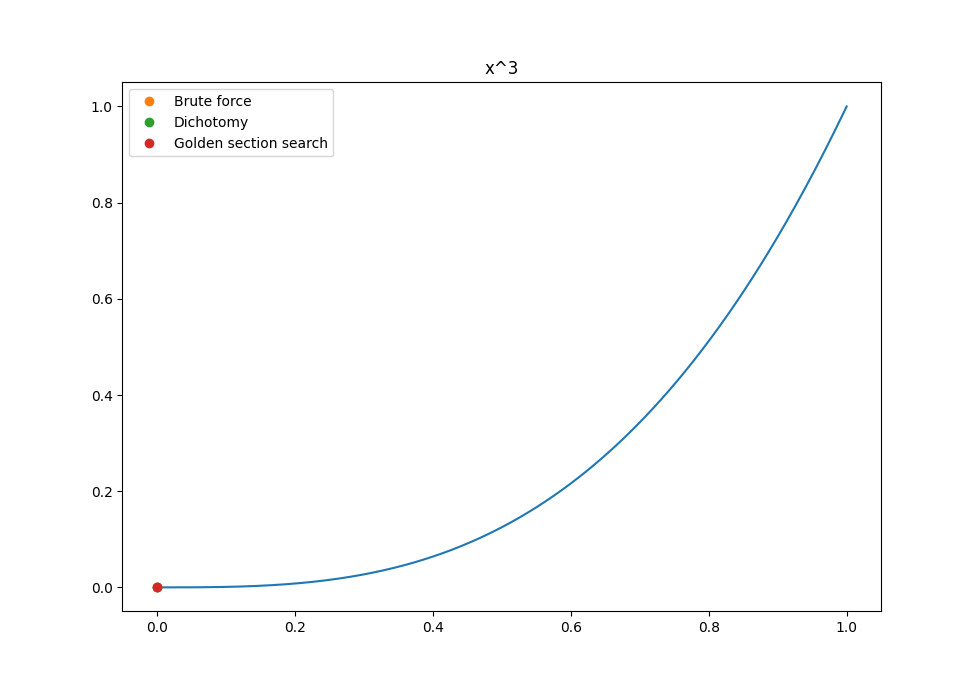
\includegraphics[width=0.7\textwidth]{../results/x_3.png}
    \captionof{figure}{$f(x) = x^3$ function minimization}
\end{center} 

\begin{table*}[h!]
    \begin{center}
        \caption{Optimization results on $f(x) = x^3$}
        \begin{tabular}{|c|c|c|c|c|}
            \textbf{Algorithm} & \textbf{$x$} & \textbf{$f(x)$} & \textbf{Evaluations} & \textbf{Iterations}\\
            \hline
            Real minimum & 0 & 0 & &\\
            Brute-force & 0.0005 & 1.25e-10 & 1000 & 1000 \\
            Dichotomy & 0.0003 & 2.38e-11 & 22 & 11 \\
            Golden-section search & 0.0004 & 4.93e-11 & 17 & 15
        \end{tabular}
    \end{center}
\end{table*}

\begin{center}
    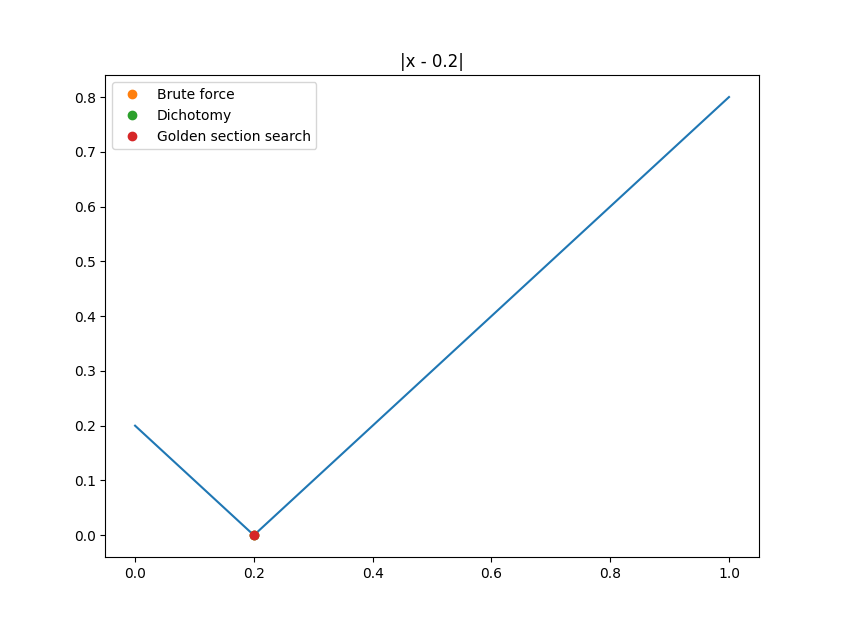
\includegraphics[width=0.7\textwidth]{../results/abs.png}
    \captionof{figure}{$f(x) = |x - 0.2|$ function minimization}
\end{center}

\begin{table*}[h!]
    \begin{center}
        \caption{Optimization results on $f(x) = |x - 0.2|$}
        \begin{tabular}{|c|c|c|c|c|}
            \textbf{Algorithm} & \textbf{$x$} & \textbf{$f(x)$} & \textbf{Evaluations} & \textbf{Iterations}\\
            \hline
            Real minimum & 0.2 & 0 & &\\
            Brute-force & 0.2005 & 0.0005 & 1000 & 1000 \\
            Dichotomy & 0.1999 & 2.27e-05 & 22 & 11 \\
            Golden-section search & 0.2001 & 7.33e-05 & 17 & 15
        \end{tabular}
    \end{center}
\end{table*}


\begin{center}
    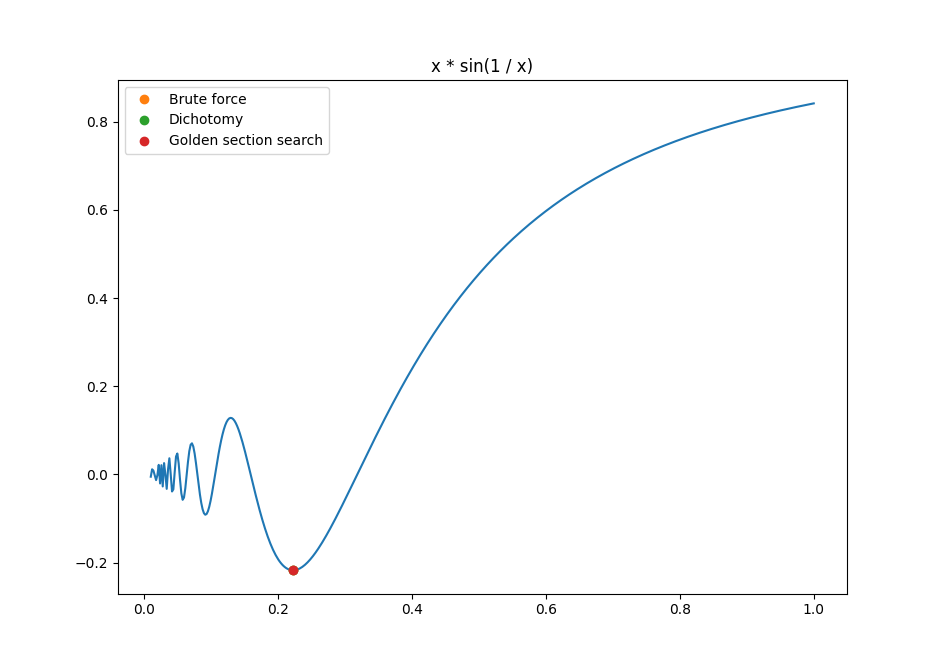
\includegraphics[width=0.7\textwidth]{../results/xsin.png}
    \captionof{figure}{$f(x) = x sin \frac{1}{x}$ function minimization}
\end{center}

\begin{table*}[h!]
    \begin{center}
        \caption{Optimization results on $f(x) = x sin\frac{1}{x}$}
        \begin{tabular}{|c|c|c|c|c|}
            \textbf{Algorithm} & \textbf{$x$} & \textbf{$f(x)$} & \textbf{Evaluations} & \textbf{Iterations}\\
            \hline
            Real minimum & 0.2225 & 0 & &\\
            Brute-force & 0.2235 & -0.2171 & 990 & 990 \\
            Dichotomy & 0.2225 & -0.2172 & 22 & 11 \\
            Golden-section search & 0.2227 & -0.2172 & 17 & 15
        \end{tabular}
    \end{center}
\end{table*}

For all functions the minimum point was found with given precision of $\epsilon = 0.001$. However, the last function does not meet requirements for
dichotomy and golden section methods (it is not convex on $[1;1]$), its form and initial bounds allows method to find minimum.

As it seen from results tables golden-section method is the most effective in terms of function evaluation counts. It require slightly more iterations then dichotomy method (its iteration count depends on delta value).
Brute-force method requires the most calculations.

\subsection*{Multidimensional optimization}

\begin{center}
    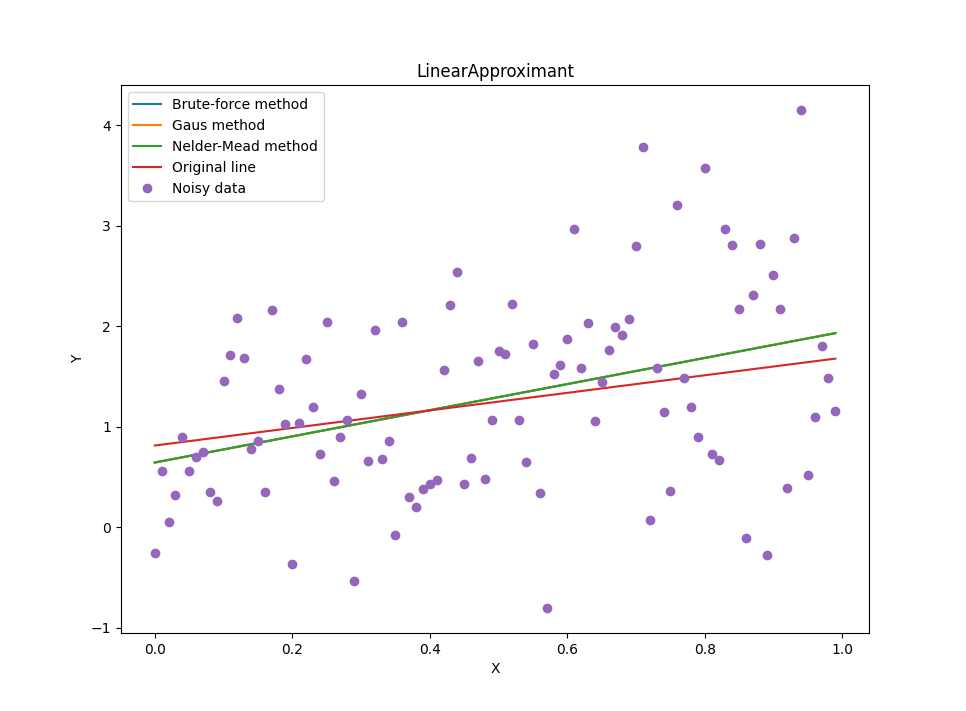
\includegraphics[width=0.7\textwidth]{../results/linear.png}
    \captionof{figure}{Linear approximant}
\end{center}

\begin{center}
    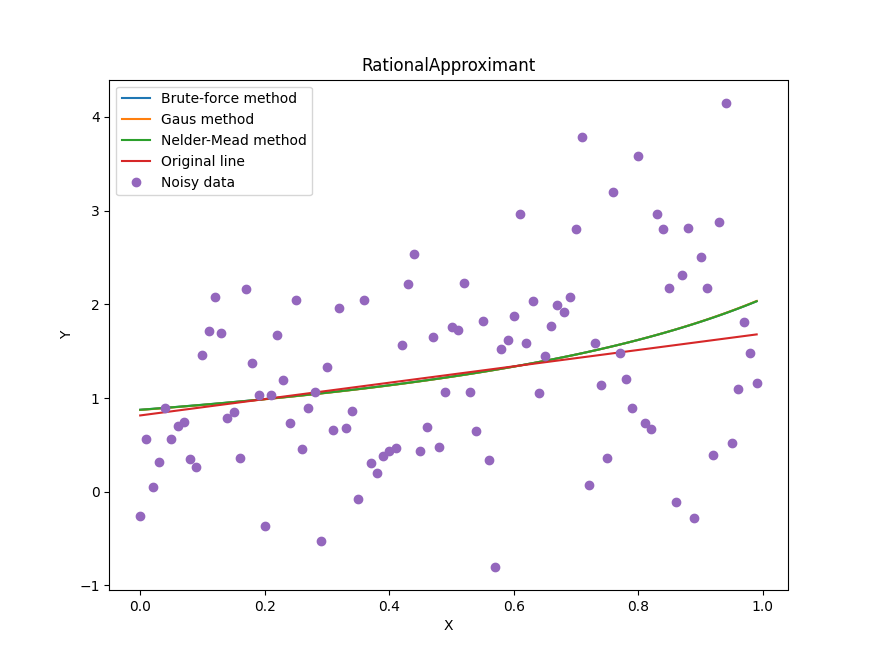
\includegraphics[width=0.7\textwidth]{../results/rational.png}
    \captionof{figure}{Rational approximant}
\end{center}

For both approximants all optimizers finds similar sollutions, although the particular found sollution depends 
on initial values (for Nelder-Mead method) and initial bounds (for brute-force and Gauss method).

\begin{table*}[h!]
    \begin{center}
        \caption{Optimization results on least squares method on bounds [0.0, 1.5], [0.0, 1.5]}
        \begin{tabular}{|c|c|c|c|c|}
            \textbf{Algorithm} & \textbf{$a, b$} & \textbf{$(\hat{y} - y)^2$} & \textbf{Evaluations} & \textbf{Iterations}\\
            \hline
            Real & (0.87, 0.81) & 82.36 & &\\
            Brute-force & (1.3004, 0.6455) & 80.6719 & 2253001 & 2253001 \\
            Gauss & (1.3028, 0.6434) & 80.6719 & 864 & 800 \\
            Nelder-Mead & (1.3000, 0.6448) & 80.6719 & 117 & 60
        \end{tabular}
    \end{center}
\end{table*}


Similarly to one-dimensional case the brute-force requires the most calculations. Nelder-Mead has the least count of function evaluations and iterations, although Gauss method (with use of golden-section method for one-dimensional optimization) has lower evaluations to iterations ratio.


	\section*{Conclusion}

In this work direct methods and metaheuristic methods was used for unconstrained non-linear optimization task. 
According to observed results it can be said that metaheuristic methods as well as direct methods can be used
in optimization when it is not possible to use higher order methods because of unavailability of derivatives. Although,
metaheuristic are usually require more computations and as well as direct methods can converge to local optima.

As well as that metaheuristic methods can be used for descreate optimization i.e in Travelling Salesman Problem. In that work,
the Simulated annealing algorithm was used for solving TSP on Western Germany cities. The results showed that usage metaheuristic methods
can significantly decrease number of computations while receiving adequate sollutions.
	\section*{Appendix}

In the next listing the implementations of used algorithms are given

\lstinputlisting{../src/optimizer.py}

In the next listing the implementation of approximants algorithms is given.

\lstinputlisting{../src/approximant.py}

For further information on code used in work and obtained results see \href{https://github.com/RyazMax/ITMO_Algorithms/tree/main/LR2}{GitHub repo}
\end{document}